% !TeX root = ../report.tex
When calculating the coordinates of the intersection points, due to the limit of float number precision, some errors might occur. In this case, a positive constant $\epsilon$ is introduced into the model. If a number is less than $\varepsilon$ or greater than $-\varepsilon$, it is regarded to be $0$. For example, to prove that a point $p_1$ is on a plane $P$, one needs to the line formed by the point $p_1$ and an arbitrary point on the plane $p_2$ is perpendicular to the normal vector $n$ of plane $P$. When defining the plane, a member variable named $p$ is assigned, in this case, $p$ is chosen as $p_2$. For various reasons such as that the normal vector of the line $L$ is normalized to length $1$, the dot product of $n$ and vector $\vec{p_1p_2}$ is not 0 but a number very close to 0. In other words, even if the point should be on the plane if calculated by hand, the answer from the computer program might not be so.

Since all of the precision problems occur in vector calculation, a special class \texttt{Vec3} is implemented with $\varepsilon$ in consideration. Experiments shows that the $\varepsilon=1^{-10}$ is an approperiate value for the HIFU simulation.

\begin{lstlisting}[language=Python]
def are_equal(a, b):
    # if the vectors a and b are equal, return True
    return all(np.abs(a - b) < EPS)

def are_parallel(a, b):
    # if the vectors a and b are parallel, return True
    reture all(np.cross(a, b) < EPS)
\end{lstlisting}

Another problem arises in the sampling phase. Given the coordinates of the intersection between the power ray of a trident ray and a sampling box, one should be able to find the index of the entry box and the exit point. However, because of the problem of float number precision, simply flooring the ratio of the offset to the length of cube edge might not always give the correct result. For example, in Figure \ref{fig:eps_handling}, there are two cases. 

\begin{figure}[h]
    \centering
    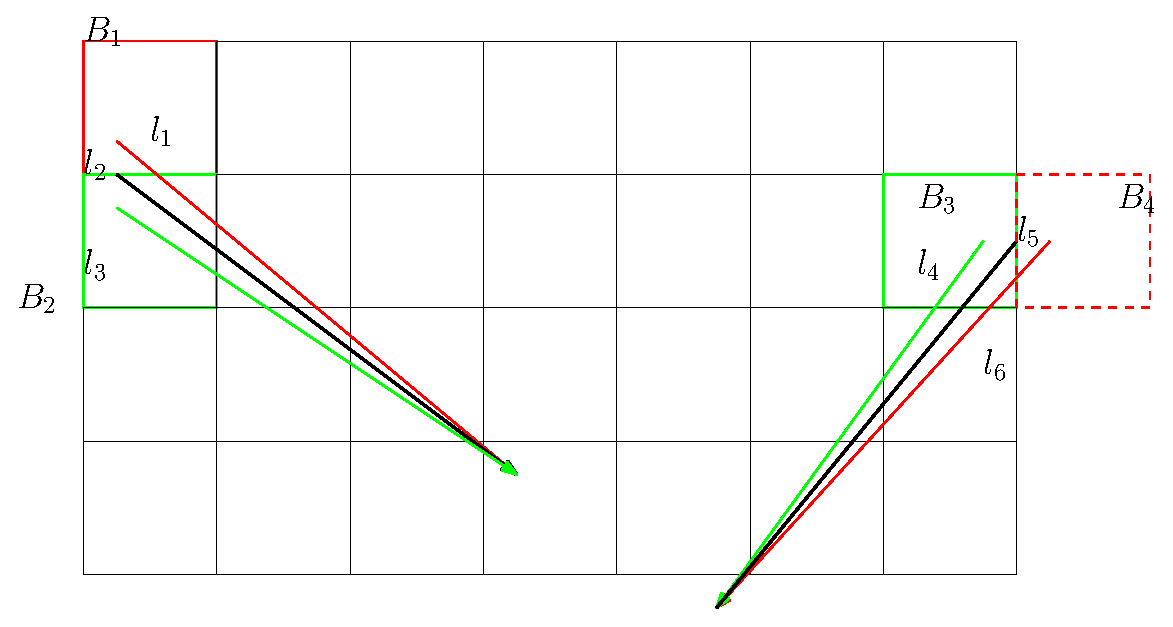
\includegraphics[width=0.65\textwidth]{ap_eps}
    \caption{Two examples of intersection with sampling box, the black lines, the green lines and the red lines are the line represented in the computer memory with errors.}
    \label{fig:eps_handling}
\end{figure}

First, suppose $l_2$ is the actual line lying exactly on the cube face. It is represented in the computer memory as $l_1$, whose starting point is in $B_1$, with the distance to the lower face of $B_1$ being $\varepsilon$. In this case, the correct entry cube is $B_2$. However, the ratio of the offset to the edge length is $\frac{1-\varepsilon}{1}$, which will be floored to 0. This gives a wrong entry box $B_1$. Second, real line $l_2$ is represented in computer memory as $l_3$, whose starting point is $\varepsilon$ away from the upper face of $B_2$. Flooring $\frac{1+\varepsilon}{1}$ would give the corret result. Now let's take a look at the right part of Figure \ref{fig:eps_handling}. Similarly, $l_5$ is the actual line mathematically. If it is represented as $l_4$ in computer memory, the result would be correct. If it is represented as $l_6$, the entry point would be $B_4$. Of course, if the actual ray is enough far away from the cube faces, there's no need to consider this float precision problem.

This problem can be solve by rounding the ratio according to the direction of the ray. Each case of green representation and red representation would be handled separately.

\IncMargin{1em}
\begin{algorithm}[H] \label{algo:properdivide}
    \DontPrintSemicolon
    \SetKwInOut{Input}{Input}\SetKwInOut{Output}{Output}
    \Input{a: $x$ coordinate of entry point, b: length of x dimension of cube, s: symbol of direction on $x$ dimension}
    \Output{\textcolor{red}{TODO}}
    r = a \% b\;
    q = a // b\;
    \uIf{$0<r<\varepsilon$}{
        \uIf{s<0}{
            $q \leftarrow q - 1$\;
            $r \leftarrow b$\;
        }
        \Else{
            $r \leftarrow 0$\;
        }
    }
    \uElseIf{$b-r<\varepsilon$}{
        \uIf{s>0}{
            $q \leftarrow q + 1$\;
            $r \leftarrow b$\;
        }
        \Else{
            $r \leftarrow 0$\;
        }
    }

    \caption{Routine of rounding $x$ dimension of entry point.}
\end{algorithm}
\DecMargin{1em}

The method to round the end point is just the opposite of that of the entry point.
